\section{Zielsetzung}
In diesem Experiment wurde die thermische Elektronenemmission anhand einer Hochvakuum-Diode untersucht. Dazu wurde insbesondere die 
Kennlinie der Diode für mehrere Heizspannungen aufgenommen.
\section{Theorie}
Neben dem photoelektrischen Effekt und der Sekundärelektronen-Emmission ist eine wesentliche Methode zur Erzeugung freier Elektronen der
sogenannte Glühelektrische Effekt, bei welchem Elektronen durch Erhitzung eines Drahtes aus selbigem austreten können. \\
Innerhalb von Metallen sorgen freie Elektronen in einem periodischen Gitter aus Ionen für die elektrische Leitfähigkeit. Das Potential 
kann in diesem Gitter näherungsweise als konstant angenommen werden und unterscheidet sich um den Wert $\Phi$ vom äußeren Potential.
Dadurch befinden sich die freien Elektronen in einem sogenannten Potentialtopf, aus dem sie nur unter Aufbringung der Austrittsarbeit
$e_0\Phi$ austreten können. \\
Die freien Elektronen unterliegen dem Pauli-Verbot, welches besagt, dass ein Energiezustand jeweils nur von zwei Elektronen mit entgegengesetzten 
Spinquantenzahlen eingenommen werden kann. Aus diesem folgt, dass die Elektronen selbst für $T=0$ eine endliche Energie besitzen. 
Die maximale Energie auf dem absoluten Nullpunkt wird als fermische Grenzenergie $\zeta$ bezeichnet. Daher müssen Elektronen, um aus dem Potentialtopf
zu gelangen und die Metalloberfläche zu verlassen, mindestens die Energie
\begin{equation}
E=\zeta+e_0\Phi
\end{equation}
besitzen. Die Wahrscheinlichkeit, dass bei einer bestimmten Themparatur eine Energiezustand besetzt ist wird durch die 
Fermi-Diracsche-Verteilungsfunktion beschrieben. Sie lautet in Näherung für große Energien:
\begin{equation}
f(E)=\exp(\frac{\zeta-E}{kT})
\end{equation}
Hier handelt es sich bei $T$ um die Temparatur und $k$ um die sogenannte Bolzman-Konstante. \\
Ausgehend von dieser Verteilung kann die Sättigungsstromdichte $J_s(T)$, also die Zahl der pro Flächen- und Zeiteinheit aus der Metalloberfläche
austretenden Elektronen in Abhängigkeit von der Temparatur, bestimmen. Durch Integration ergibt sich nach längerer Rechnung für diesen Wert die sogenannte
Richardson Gleichung
\begin{equation}
    \label{eq:richardson}
J_s(T)=4\pi\frac{e_0m_0k^2}{h^3}T^2\exp(\frac{-e_0\Phi}{kT})
\end{equation}
wobei die Elementarladung $e_0$, die Elektronenmasse $m_0$ und das Plancksche Wirkungsquantum $h$ allesamt Konstanten bezeichnen. \\
Die Messung des Sättigungsstromes erfolgt in einer Hochvakuum Diode.
\begin{figure}[h]
    \centering
    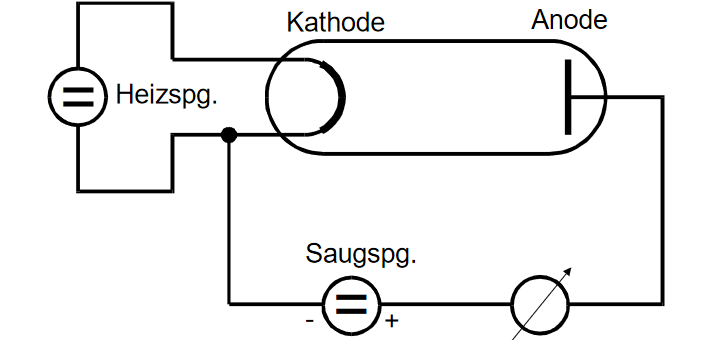
\includegraphics[width=4cm, keepaspectratio]{Hochvakuum-Diode}
    \label{Drehimpuls}
  \end{figure}
Diese besteht aus einer evakuirten Röhre, in der ein Draht mithilfe einer
Heizspannung erhitzt wird. Die aus der Kathode austretenden Elektronen werden mittels einer Saugspannung zur Anode hin beschleunigt
und der resultierende Strom gemessen. Das Vakuum ist dabei essentiell, das die Elektronen ansonsten durch Wechselwirkung mit den Luftmolekülen nicht 
bis zur Anode gelangen würden. \\
Bei einer Strommessung mit einer entsprechenden Vorrichtung ist auffällig, dass sich erst ab einer hinreichen hohen Saugspannug 
der nach der Richardson-Gleichung zu erwartende Sättigungsstrom einstellt. Dies liegt daran, dass die Bewegung der Elektronen beschleunigt ist,
die Elektronen also nahe der Kathode sehr viel langsamer als nahe der Anode sind. Daraus resultiert eine negative Raumladung vor der Kathode,
die diese vom durch die Saugspannung induzierten elektrischen Feld abschirmt. Da die Feldlinien des äußeren Feldes also an den Raumladungselektronen 
und an der Kathode enden, werden einige Elektronen nicht erfasst und der Anodenstrom wird verringert.
Ausgehend von der Poissongleichung in einer Dimension 
\begin{equation}
\frac{d^2}{dx^2}V=-\frac{\rho}{\epsilon_0}
\end{equation}
mit der Raumladungsdichte $\rho$ kann hergeleitet werden, dass das Potential unter Berücksichtigung der Raumladung eine $x^{\frac{4}{3}}$ besitzt, 
anstelle eines linearen anwachsenden Potentials im Raumladungsfreien Fall, woraus folgt, dass das Elektrische Feld proportional zu $x^{\frac{1}{3}}$
und die Raumladungsdichte proportional zu $x^{-\frac{2}{3}}$ verläuft. Daraus lässt sich für den Zusammenhang zwischen der Stromdichte $j$ 
und der Anodenspannung $U$ das Langmuir-Schottkysche Raumladungsgesetz 
\begin{equation}
j=\frac{4}{9}\epsilon_0\sqrt{2e_0/m_0}\frac{U^{\frac{3}{2}}}{a^2}
\end{equation}
herleiten. Hier beschreibt $a$ den Abstand zwischen Anode und Kathode. \\
Jede Hochvakuum-Diode verfügt über eine Kennlinie, die den Anodenstrom in Abhängigkeit von der Saugspannung beschreibt. Diese Kennlinie lässt 
sich in drei Abschnitte gliedern und nimmt in aller Regel folgende Form an:
\begin{figure}[h]
    \centering
    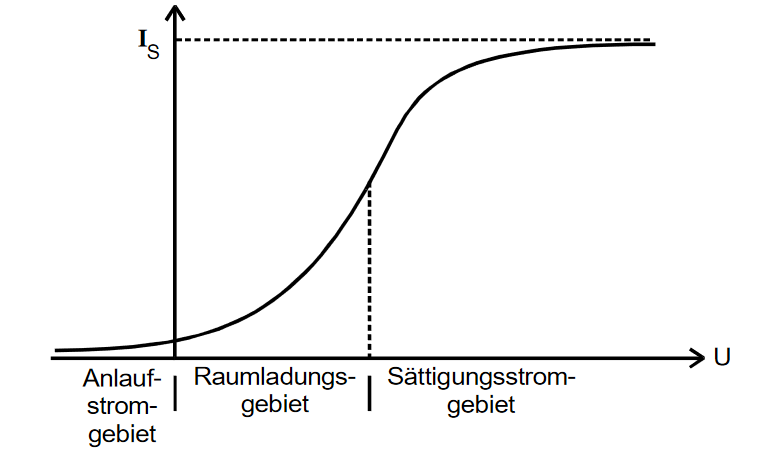
\includegraphics[width=4cm, keepaspectratio]{Kennlinie}
    \label{Drehimpuls}
  \end{figure}
Hier ist auffällig, dass auch ohne Saugspannung bereits ein Anodenstrom Auftritt. Dieses Phänomen ist darauf zurückzuführen, 
dass die aus der Kathode austretenden Elektronen die Differenz zwischen ihrer ursprünglichen Energie und der zum Austritt aus dem Material benötigten Energie
\begin{equation}
\Delta E=E-\zeta+e_0\Phi
\end{equation}
in Form kinetischer Energie behalten, welche ausreicht selbst gegen ein geringes Gegenfeld zur Anode zu gelangen. Dieser Bereich der Kennlinie wird als
Anlaufstrombereich bezeichnet. In diesem lässt sich die Stromdichte durch den exponentiellen Zusammenhang
\begin{equation}
j=const\exp(-\frac{e_0U}{kT})
\end{equation}
beschreiben. An das Anlaufstromgebiet schließt sich das Raumladungsgebiet an, in dem das Langmuir-Schottkysche Raumladungsgesetz gilt. Mit steigender
Anodenspannung wird dieses schließlich vom Sättigungsstromgebiet abgelöst, in dem sich der Anodenstrom asymptotisch dem durch die Richardson-Gleichung
festgelegten Grenzwert nähert.


